\section{Physical Simulation}

\subsection{Dynamics Equation}

We model the robot as an articulated rigid body system in our simulator, which satisfies the following dynamics equations, non-penetration and linear complementarity conditions for contact points.

\begin{align}
\label{eq:robotdynamics}
\mathbf{M}(\mathbf{q})\mathbf{\ddot{q}}+\mathbf{C}(\mathbf{q},\mathbf{\dot{q}})&=\boldsymbol{\tau}+\mathbf{J}(\mathbf{q})^T\mathbf{f}\\
\nonumber \mathbf{d}(\mathbf{q})&\geq \mathbf{0}\\
\nonumber \mathbf{d}(\mathbf{q})^T\mathbf{f}&= \mathbf{0}\\
\nonumber \mathbf{f}&\in\mathbf{K}
\nonumber \end{align}

where $\mathbf{M}(\mathbf{q})$ is the mass matrix and $\mathbf{C}(\mathbf{q},\mathbf{\dot{q}})$ is the Coriolis and Centrifugal force. $\boldsymbol{\tau}$ are joint torques exerted by the actuators. An actuator model that computes $\boldsymbol{\tau}$ based on the current state and a reference trajectory is presented in the next section. $\mathbf{J}(\mathbf{q})$ is the Jacobian matrix and $\mathbf{f}$ is the contact force. $\mathbf{d}(\mathbf{q})$ is the distance of the contact to the ground and $\mathbf{K}$ is the friction cone. In our implementation, we solve a velocity-based LCP problem to compute $\mathbf{f}$, $\mathbf{q}$ and $\dot{\mathbf{q}}$ simultaneously using DART. Please refer to the tutorial of the LCP formulation \cite{Tan:2012b} for futher details.
\ignorethis{
  /karen{Make actuator modeling sound important. Argue why we had to build an accurate model for actuator instead of improving other sources of simulation errors.}
  }

\subsection{Actuator Model}
\label{sec:motorDynamics}
A faithful robot simulation relies heavily on an accurate actuator model. A common practice is to set the same PID gains in the simulation as those in the servo. However, Dynamixel AX-18 servos, used on our robot (ROBOTIS BIOLOID GP), do not support PID control. Although the servo can track an input desired angle $\bar{q}$, the relation between the joint error $\bar{q}-q$ and the output torque $\tau$ is unclear. We derive an actuator model based on the ideal DC motor assumption and the specification of the servo:

\begin{equation}
  \tau = -k_p(q-\bar{q}) - k_d\dot{q} - k_c\sgn(\dot{q})\\
    \label{eqn:torqueErrorRelationSimple}
\end{equation}
We call $k_p$, $k_d$ and $k_c$ the \emph{actuator gains}. Note that these are not PID gains. These gains are determined by the design of the servo, which are unknown to us. The detailed derivation of the actuator model (eq. (\ref{eqn:torqueErrorRelationSimple})) can be found in Appendix.

Accurately identifying these gains would be difficult and tedious, requiring a large number of carefully designed experiments on each of the actuators. Instead, we choose to run only one simple experiment on one actuator. This gives us an initial guess of the gains. We then rely on simulation calibration to refine this estimation.

In the experiment, we clamp the entire robot on a table except for the left foot. We then send a periodic control signal $\bar{q}(t)$ to the servo at the left ankle (blue curve in Figure \ref{fig:actuatorId}). The desired joint angle stays at the maximum value for 0.67 second, then changes to the minimum value and stays for another 0.67 second and repeats. We record the trajectory of the actual joint angle $q(t)$ throughout the experiment (green curve in Figure \ref{fig:actuatorId}). 

\begin{figure}[!t]
  \centering
  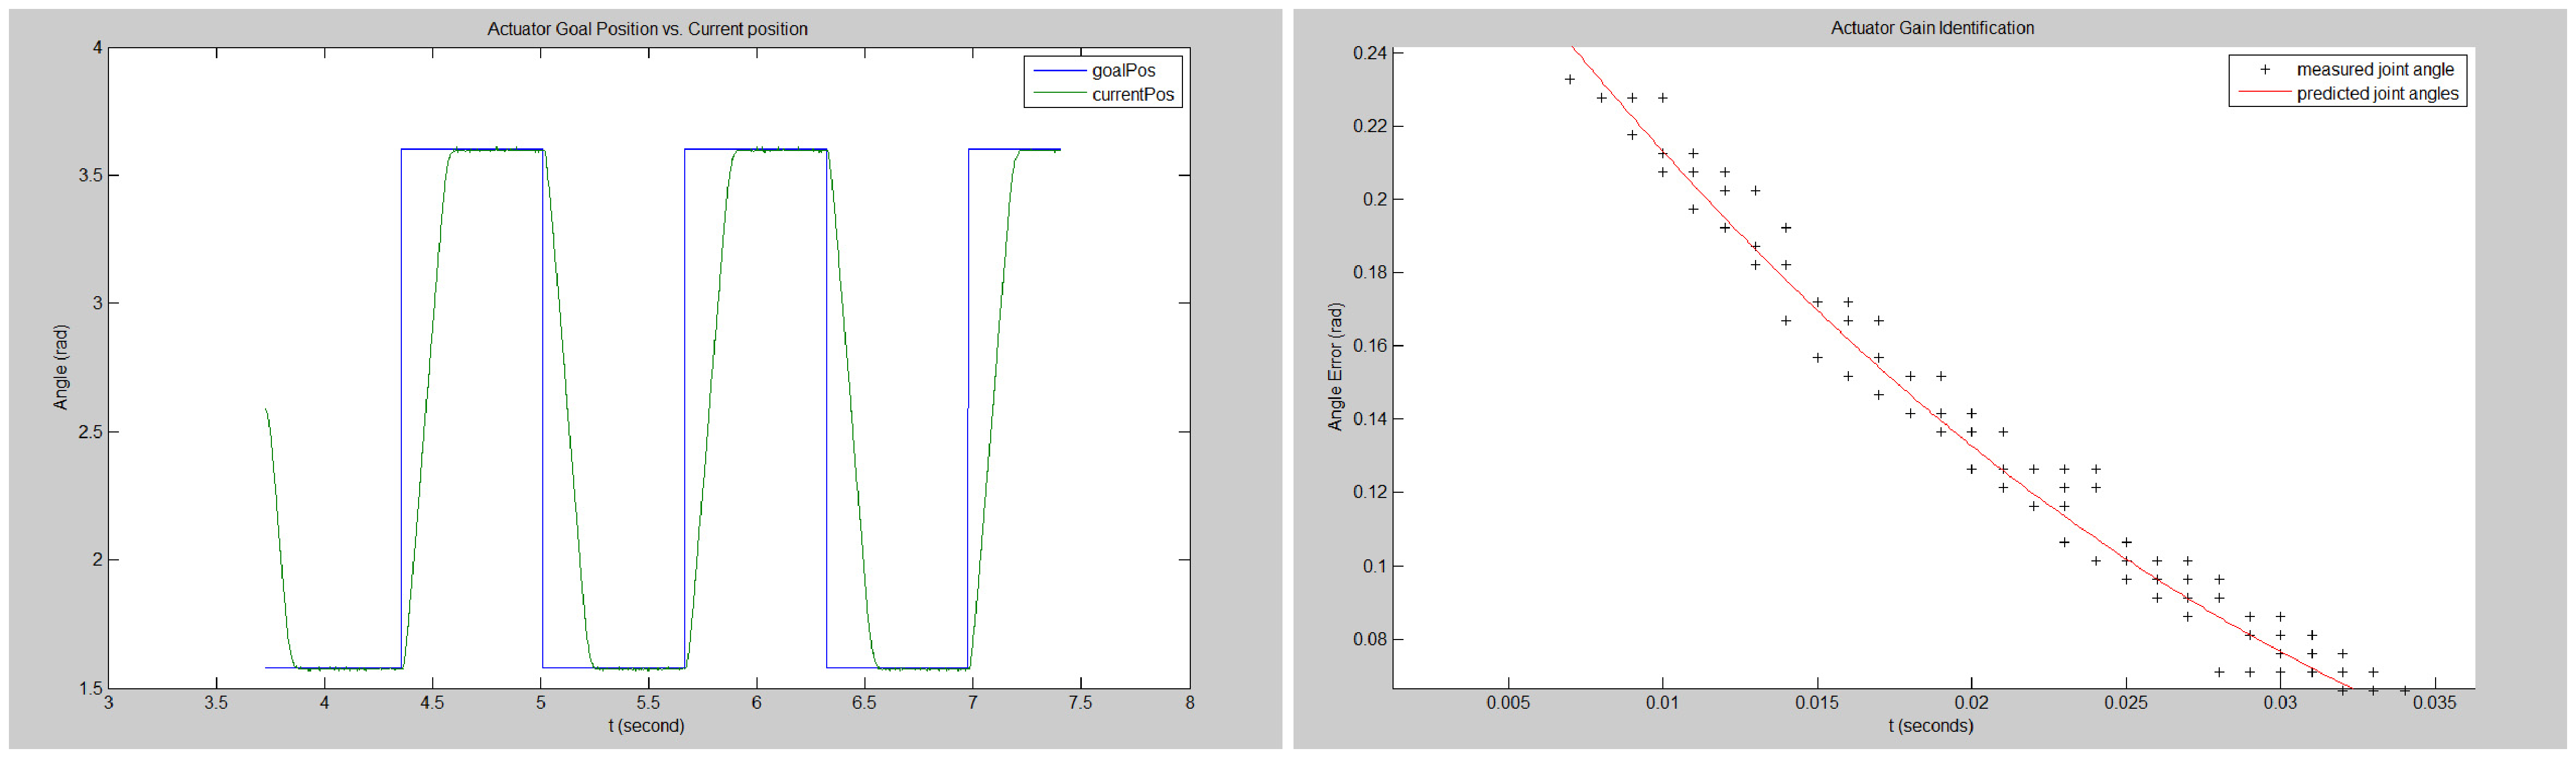
\includegraphics[width=0.3\textwidth]{figures/actuatorId}
  \caption{The trajectories of the desired and the measured joint angle for acutator identification.}
  \vspace{-0.1in}
  \label{fig:actuatorId}
\end{figure}

Given $q(t)$ and $\bar{q}(t)$, we apply regression to estimate the actuator gains:

\begin{displaymath}
\min_{k_p, k_d, k_c}\int||I\ddot{q}(t)+k_p(q(t)-\bar{q}(t)) + k_d\dot{q}(t) + k_c\sgn(\dot{q}(t))||^2\mathrm{d}t
\end{displaymath}
where $I$ is the moment of inertia of the foot with respect to the rotating axis. The above equation is derived by plugging into $\tau = I\ddot{q}+\dot{I}\dot{q}$ and the fact that $\dot{I}\dot{q}=0$ because the foot is a rigid body that rotates along a fixed axis. Our experiments and computation show that the actuator gains are $k_p=9.272(N\cdot m/rad)$, $k_d=0.3069(N\cdot m\cdot s/rad)$, and $k_c=0.03(N\cdot m)$. 



%\begin{displaymath}
%\min_{\boldsymbol{\theta}}\frac{1}{n}\sum_{i=1}^{n}\int||\tilde{\mathbf{x}}_i(\bar{\mathbf{q}}(t))-\mathbf{x}(\bar{\mathbf{q}}(t);\boldsymbol{\theta})||^2\mathrm{d}t
%\end{displaymath}
